\documentclass[a4paper,12pt]{article}
%%%%%%%%%%%%%%%%%%%%%%%%%%%%%%%%%%%%%%%%%%%%%%%%%%%%%%%%%%%%%%%%%%%%%%%%%%%%%%%%%%%%%%%%%%%%%%%%%%%%%%%%%%%%%%%%%%%%%%%%%%%%%%%%%%%%%%%%%%%%%%%%%%%%%%%%%%%%%%%%%%%%%%%%%%%%%%%%%%%%%%%%%%%%%%%%%%%%%%%%%%%%%%%%%%%%%%%%%%%%%%%%%%%%%%%%%%%%%%%%%%%%%%%%%%%%
\usepackage{eurosym}
\usepackage{vmargin}
\usepackage{amsmath}
\usepackage{graphics}
\usepackage{epsfig}
\usepackage{framed}
\usepackage{subfigure}
\usepackage{fancyhdr}

\setcounter{MaxMatrixCols}{10}
%TCIDATA{OutputFilter=LATEX.DLL}
%TCIDATA{Version=5.00.0.2570}
%TCIDATA{<META NAME="SaveForMode"CONTENT="1">}
%TCIDATA{LastRevised=Wednesday, February 23, 201113:24:34}
%TCIDATA{<META NAME="GraphicsSave" CONTENT="32">}
%TCIDATA{Language=American English}

\pagestyle{fancy}
\setmarginsrb{20mm}{0mm}{20mm}{25mm}{12mm}{11mm}{0mm}{11mm}
\lhead{Advanced Data Modelling} \rhead{Logistic Regression} \chead{MA4128} %\input{tcilatex}

%http://www.electronics.dit.ie/staff/ysemenova/Opto2/CO_IntroLab.pdf
\begin{document}

\tableofcontents

	%----------------------------------------------------------------------------------------%
	
	\begin{framed}
		\subsection*{Types of Variables (Revision)}
		\begin{itemize}
			\item Examples of \textbf{continuous variables} include revision time (measured in hours), intelligence (measured using IQ score), exam performance (measured from 0 to 100), weight (measured in kg), and so forth. 
			
			\item Examples of \textbf{ordinal variables} include \textit{Likert} items (e.g., a 7-point scale from "strongly agree" through to "strongly disagree"), amongst other ways of ranking categories (e.g., a 3-point scale explaining how much a customer liked a product, ranging from "Not very much" to "Yes, a lot"). 
			\item Examples of \textbf{nominal variables} include gender (e.g., 2 groups: male and female), ethnicity (e.g., 3 groups: Caucasian, African American and Hispanic), profession (e.g., 5 groups: surgeon, doctor, nurse, dentist, therapist), and so forth.
		\end{itemize}
	\end{framed}
	
	
	
	
	\subsection*{South Africa Heart Disease Data Example}
	
	\begin{framed}
		A retrospective sample of males in a heart-disease high-risk region
		of the Western Cape, South Africa. There are roughly two controls per
		case of CHD. Many of the CHD positive men have undergone blood
		pressure reduction treatment and other programs to reduce their risk
		factors after their CHD event. In some cases the measurements were
		made after these treatments. These data are taken from a larger
		dataset, described in  Rousseauw et al, 1983, South African Medical
		Journal. 
		
	\end{framed}
	%Load the South Africa Heart Disease Data and create training and test sets with
	%the following code:
	%\begin{framed}
	%	\begin{verbatim}
	%	install.packages("ElemStatLearn")
	%	library(ElemStatLearn)
	%	data(SAheart)
	%	
	%	set.seed(8484)
	%	train = sample(1:dim(SAheart)[1],
	%	size=dim(SAheart)[1]/2,replace=F)
	%	trainSA = SAheart[train,]
	%	testSA = SAheart[-train,]
	%	
	%	\end{verbatim}
	%\end{framed}
	
	\noindent \textbf{Exercise}\\Fit a logistic regression model with
	\begin{itemize}
		\item \textit{Coronary Heart Disease} (\texttt{chd}) as the
		dependent variable
		
		\item \textit{age at onset, current alcohol consumption, obesity levels,
			cumulative tabacco, type-A behavior}, and \textit{low density lipoprotein cholesterol} as predictor variables. 
	\end{itemize} 
	{
		\large
		
		\begin{verbatim}
		> head(SAheart)
		sbp tobacco  ldl adiposity famhist typea obesity alcohol age chd
		1 160   12.00 5.73     23.11 Present    49   25.30   97.20  52   1
		2 144    0.01 4.41     28.61  Absent    55   28.87    2.06  63   1
		3 118    0.08 3.48     32.28 Present    52   29.14    3.81  46   0
		4 170    7.50 6.41     38.03 Present    51   31.99   24.26  58   1
		5 134   13.60 3.50     27.78 Present    60   25.99   57.34  49   1
		6 132    6.20 6.47     36.21 Present    62   30.77   14.14  45   0
		...
		...
		\end{verbatim}
		
	}
	\noindent Calculate the misclassification rate for your model using this model
	% function and a prediction on the "response" scale:
	
	%\noindent What is the misclassification rate on the training set? What is the
	%misclassification rate on the test set?
	%\begin{framed}
	%	\begin{verbatim}
	%	head(SAheart)
	%	
	%	lr1 <- glm(chd ~ age + alcohol + obesity + 
	%	tobacco + typea + ldl, data=trainSA, 
	%	family="binomial")
	%	
	%	lr1.train.predict <- predict(lr1, type="response")
	%	
	%	missclass.lr1.train <- missClass(trainSA$chd, 
	%	lr1.train.predict)
	%	
	%	lr1.test.predict <- predict(lr1, newdata=testSA, 
	%	type="response")
	%	
	%	missclass.lr1.test <- missClass(testSA$chd, 
	%	lr1.test.predict)
	%	\end{verbatim}
	%\end{framed}
	
	
	\newpage
	%-------------------------------------------------------%
	
	%------------------------------------------------------------------------------------%

	\section{Review of Logistic Regression}
	% http://www.nesug.org/proceedings/nesug06/an/da26.pdf
	% http://www.ccsr.ac.uk/publications/teaching/blr.pdf
	% http://www.southampton.ac.uk/ghp3/docs/unicef/presentation7.1a.pdf
	% ftp://public.dhe.ibm.com/software/analytics/spss/documentation/statistics/20.0/en/client/Manuals/IBM_SPSS_Regression.pdf
	% http://www.umass.edu/statdata/statdata/data/
		
	\subsection*{Logistic Regression: Logit Transformation}
	%http://data.princeton.edu/wws509/notes/c3.pdf
	
	The logit transformation is given by the following formula: 
	\[ \eta_i = \mbox{logit}(\pi_i)  = \mbox{log}\left( \frac{\pi_i}{1- \pi_i} \right) \]
	
	\noindent 
	The inverse of the logit transformation is given by the following formula: 
	\[ \pi_i = \mbox{logit}^{-1}(\eta_i)  =  \frac{e^{\eta_i}}{1 + e^{\eta_i}} \]
	
	%---------------------------%


\subsection{Dummy variables}
When an explanatory variable is categorical we can use \textbf{dummy variables} to contrast
the different categories. For each variable we choose a baseline category and then
contrast all remaining categories with the base line. If an explanatory variable
has k categories, we need k-1 dummy variables to investigate all the differences in
the categories with respect to the dependent variable.

For example suppose the explanatory variable was \textbf{\textit{housing}} coded like this:
\begin{itemize}
	\item[1:] Owner occupier
	\item[2:] renting from a private landlord
	\item[3:] renting from the local authority
\end{itemize}

We would therefore need to choose a baseline category and create two dummy
variables. For example if we chose owner occupier as the baseline category we
would code the dummy variables (House1 and House2) like this

%Tenure: &House1 &House2\\
%Owner occupier &0& 0\\
%Rented private &1 &0\\
%Rented local authority &0 &1\\

%%%%%%%%%%%%%%%%%%%%%%%%%%%%%%%%%%%%%%%%%%%%%%%%%%%%%%%%%%%%%%%%%%%%%%%%%%%%%%%%%%%%%%%%%%%%%%%%%%%5




\section*{Introduction to Logistic Regression}

The term �\textbf{\textit{generalized linear model}}� is used to describe a procedure for
transforming the dependent variable so that the �right hand side� of the model
equation can be interpreted as a \textbf{�\textit{linear combination}}� of the explanatory variables. 	In logistic regression, the logit may be computed in a manner similar to linear regression:
\[ \eta_i = \beta_0 + \beta_1x_1 + \beta_2x_2 + \ldots  \]

In situations where the dependent (y) variable is continuous and can be
reasonably assumed to have a normal distribution we do not transform the y
variable at all and we can simply run a multiple linear regression analysis.

Otherwise some sort of transformation is applied.


%---------------------------------------------------------------%
\subsection{Binomial Logistic Regression} 
A binomial logistic regression (often referred to simply as logistic regression), predicts the probability that an observation falls into one of two categories of a \textbf{dichotomous} dependent variable based on one or more independent variables that can be either continuous or categorical.

% \section{Binomial Logistic Regression}
Binomial logistic regression estimates the probability of an event (as an example, having heart disease) occurring. 
\begin{itemize}
	\item If the estimated probability of the event occurring is greater than or equal to 0.5 (better than even chance), the procedure classifies the event as occurring (e.g., heart disease being present). \item If the probability is less than 0.5, Logistic regression classifies the event as not occurring (e.g., no heart disease). 
\end{itemize}

\subsection{Examples of Logistic Regression}

\begin{description}
	\item[Example 1:]  Suppose that we are interested in the factors that influence whether a political candidate wins an election.  The outcome (response) variable is binary (0/1); \textit{ win or lose}.  The predictor variables of interest are the amount of money spent on the campaign, the amount of time spent campaigning negatively and whether or not the candidate is an incumbent.
	
	\item[Example 2:]  A researcher is interested in how variables, such as GRE (Graduate Record Exam scores), GPA (grade point average) and prestige of the undergraduate institution, effect admission into graduate school. The response variable, \textit{admit/don't admit}, is a binary variable.
\end{description}


\begin{framed}
	\subsection*{Types of Variables (Revision)}
	\begin{itemize}
		\item Examples of \textbf{continuous variables} include revision time (measured in hours), intelligence (measured using IQ score), exam performance (measured from 0 to 100), weight (measured in kg), and so forth. 
		
		\item Examples of \textbf{ordinal variables} include \textit{Likert} items (e.g., a 7-point scale from "strongly agree" through to "strongly disagree"), amongst other ways of ranking categories (e.g., a 3-point scale explaining how much a customer liked a product, ranging from "Not very much" to "Yes, a lot"). 
		\item Examples of \textbf{nominal variables} include gender (e.g., 2 groups: male and female), ethnicity (e.g., 3 groups: Caucasian, African American and Hispanic), profession (e.g., 5 groups: surgeon, doctor, nurse, dentist, therapist), and so forth.
	\end{itemize}
\end{framed}






\subsection*{Logistic function} 

The logistic function, with $\beta_0 + \beta_1 x$ on the horizontal axis and $\pi(x)$ on the vertical axis
An explanation of logistic regression begins with an explanation of the logistic function, which always takes on values between zero and one:
\[
F(t) = \frac{e^t}{e^t+1} = \frac{1}{1+e^{-t}},
\]
and viewing $t$ as a linear function of an explanatory variable x (or of a linear combination of explanatory variables), the logistic function can be written as:
\[\pi(x) = \frac{e^{(\beta_0 + \beta_1 x)}} {e^{(\beta_0 + \beta_1 x)} + 1} = \frac {1} {1+e^{-(\beta_0 + \beta_1 x)}}.
\]
This will be interpreted as the probability of the dependent variable equalling a ``success" or ``case" rather than a failure or non-case. We also define the inverse of the logistic function, the logit:
\[g(x) = \log \frac {\pi(x)} {1 - \pi(x)} = \beta_0 + \beta_1 x ,
\]and equivalently:
\[\frac{\pi(x)} {1 - \pi(x)} = e^{(\beta_0 + \beta_1 x)}.
\]
%======================================================%


%---------------------------%


%------------------------------------------------------------------------------------%
\section{Logistic Regression}
Logistic regression, also called a logit model, is used to model \textbf{dichotomous outcome} variables. 
In the logit model the \textbf{log odds} of the outcome is modeled as a linear combination of the predictor variables.

In logistic regression theory, the predicted dependent variable is a function of the probability that a particular subject will be in one of the categories (for example, the probability that a patient has the disease, given his or her set of scores on the predictor variables).





%-------------------------------------------%
\newpage
\subsection{Variable Selection}
Like ordinary regression, logistic regression provides a coefficient \textbf{b} estimates, which measures
each IV�s partial contribution to variations in the response variables. The goal is to correctly predict
the category of outcome for individual cases using the most parsimonious model.

To accomplish this goal, a model (i.e. an equation) is created that includes all predictor variables that are useful in predicting the response variable. Variables can, if necessary, be entered into the model in the order specified by the researcher in a stepwise fashion like regression.

There are two main uses of logistic regression:
\begin{itemize}
	\item The first is the prediction of group membership. Since logistic regression calculates the
	probability of success over the probability of failure, the results of the analysis are in
	the form of an \textbf{odds ratio}.
	\item Logistic regression also provides knowledge of the relationships and strengths among
	the variables (e.g. playing golf with the boss puts you at a higher probability for job
	promotion than undertaking five hours unpaid overtime each week).
\end{itemize}



%---------------------------------------------------------- %

\subsection{SPSS Output}
\begin{itemize}
	\item The variable Vote2005 is a binary variable describing turnout at a general election. The predictor variables are gender and age.
	\begin{center}
		\begin{figure}[h!]
			% Requires \usepackage{graphicx}
			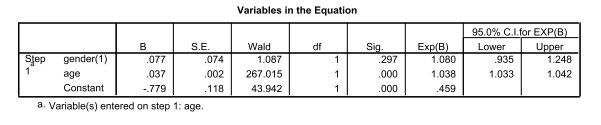
\includegraphics[scale=0.6]{LogWeek10B}\\
			\caption{General Election 2005}
		\end{figure}
	\end{center}
	
	% Image LogWeek10-B
	
	\[\mbox{logit(vote2005)} = -.779 + .077\mbox{gender(1)}+.037\mbox{age}\]
	
	\item The age coefficient is statistically significant. Exp(B) for age is 1.038, which
	means for each year different in age, the person is 1.038 times more likely to turn
	out to vote, having allowed for gender in the model. Eg. a 21 year old is 1.038
	times as likely to turn out to vote than a 20 year old. \item This might not seem much
	of a difference but a 20 year difference leads to a person being $1.038^20 = 2.11$
	times more likely to turn out to vote. E.g. a 40 year old is 2.11 times more likely to
	turn out to vote than a 20 year old, having allowed for gender in the model.
	
	
	\item The gender coefficient is not statistically significant.
	
	
\end{itemize}





\subsection{Logistic Regression: Decision Rule}
Our decision rule will take the following form: If the probability of the event is greater than or equal to some threshold, we shall predict that the event will take place. By default, SPSS sets this threshold to .5. While that seems reasonable, in many cases we may want to set it higher or lower than .5.

%---------------------------------------------------------- %




\section{Summary of Logistic Regression}
logistic regression or logit regression is a type of regression analysis used for predicting
the outcome of a categorical dependent variable (a dependent variable that can take on a limited number of values,
whose magnitudes are not meaningful but whose ordering of magnitudes may or may not be meaningful)
based on one or more predictor variables.



\begin{itemize}
	\item[(1.)] Logistic regression is intended for the modeling
	of dichotomous categorical outcomes (e.g., characterized by binary responses: buy vs Don't buy, dead vs. alive, cancer vs. none,�).
	
	
	\item[(2.)] We want to predict the probability of a particular response  (0 to 1 scale).
	
	\item[(3.)] For binary responses, linear regression should not be used for several reasons
	but the most common-sense reason is that linear regression can provide predictions NOT on a 0 to 1 scale.
	but rather a predicted response of some numeric value (e.g 2.4 or -800.3).
	
	\item[(4.)] We need a way to link the probabilistic response variable to the continuous and/or categorical predictors and
	keep things on this 0 to 1 scale.
	
	\item[(5.)] Logistic regression winds up transforming the probabilities to odds and then taking the natural logarithm of these odds, called logits.
	
	
	\item[(6.)] Suppose a response variable is passing a test (by convention, 0=no and 1=yes).
	You have 1 predictor - number of days present in class over the past 30 days.
	Suppose the regression coefficient (often just called beta) in the output is 0.14.
	You would then say that, on average, as class presence increases by 1 day, the natural logarithm of the
	odds of passing the test increases by 0.14.
	
	\item[7.)] For the interpretation, you can just talk about the odds.
	Most computer output will give you this number.
	Suppose the answer in odds is 1.24. Then, you just say that,on average, as class presence increases by 1 day,
	the odds of passing the test are multiplied by 1.24.
	In other words, for each additional day present, the odds of passing are 24% greater than that of not passing.
	
	\item[8.)] To validate our findings, normally, we test whether the regression coefficient is equal to zero in the population.
	In logistic regression, the corresponding value for the odds is one (not zero). We got an odds of 1.24.
	Can we trust this? Or should we go with one (which would mean that the odds are the same for both passing and not passing,
	and hence class presence makes no difference at all)?  Look at the p-value (significance). If it less than .05 (by convention), you have enough evidence to reject
	the notion that the odds are really one. You go ahead and support the 1.24 result.
\end{itemize}


%-------------------------------------------%





%---------------------------------------------------------- %
\subsection{Variables in the Equation}
The Variables in the Equation table has several important elements. The Wald statistic and associated probabilities provide an index of the significance of each predictor in the equation.
The simplest way to assess Wald is to take the significance values and if less
than 0.05 reject the null hypothesis as the variable does make a significant contribution.
In this case, we note that family size contributed significantly to the prediction
(p = .013) but mortgage did not (p = .075). The researcher may well want to drop
independents from the model when their effect is not significant by the Wald statistic
(in this case mortgage).

\begin{figure}
	\begin{center}
		% Requires \usepackage{graphicx}
		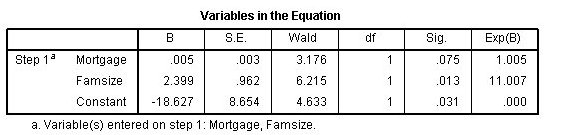
\includegraphics[scale=0.6]{images/Logistic8}\\
		\caption{Variables in the Equation}
	\end{center}
\end{figure}

The \textbf{\textit{Exp(B)}} column in the table presents the extent to which raising the corresponding measure by one unit influences the odds ratio. We can interpret \textbf{\textit{Exp(B)}}) in
terms of the change in odds. If the value exceeds 1 then the odds of an outcome occurring increase; if the figure is less than 1, any increase in the predictor leads to a drop in
the odds of the outcome occurring. For example, the \textbf{\textit{Exp(B)}} value associated with
family size is 11.007. Hence when family size is raised by one unit (one person) the
odds ratio is 11 times as large and therefore householders are 11 more times likely to
belong to the take offer group.

The \textbf{\textit{B}} values are the logistic coefficients that can be used to create a predictive
equation (similar to the b values in linear regression) formula seen previously.
\begin{figure}
	\begin{center}
		% Requires \usepackage{graphicx}
		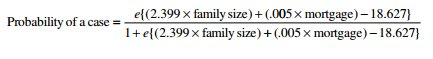
\includegraphics[scale=0.75]{images/Logistic11}\\
		\caption{Logistic Regression Equation}
	\end{center}
\end{figure}

Here is an example of the use of the predictive equation for a new case. Imagine a
householder whose household size including themselves was seven and paying
a monthly mortgage of $2,500$ euros. Would they take up the offer, i.e. belong to category 1?
Substituting in we get:
\begin{figure}
	\begin{center}
		% Requires \usepackage{graphicx}
		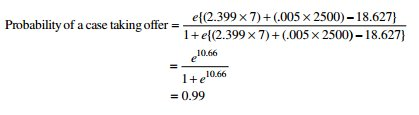
\includegraphics[scale=0.75]{images/Logistic12}\\
		\caption{Logistic Regression Equation : Example}
	\end{center}
\end{figure}

Therefore, the probability that a householder with seven in the household and a mortgage of 2,500 p.m. will take up the offer is 99\%, or 99\% of such individuals will be
expected to take up the offer.
Note that, given the non-significance of the mortgage variable, you could be justified
in leaving it out of the equation. As you can imagine, multiplying a mortgage value by
B adds a negligible amount to the prediction as its B value is so small (.005).

%%%%%%%%%%%%%%%%%%%%%%%%%%%%%%%%%%%%%%%%%%%%%%%%%%%%%%%%%%%%%%%%%%%%%%%%%%%%%%%%%%%%%%%%%%%%%%%%%%%%%%%%%%%%


\begin{itemize}
	\item[(1.)] Logistic regression is intended for the modeling
	of dichotomous categorical outcomes (e.g., characterized by binary responses: buy vs Don't buy, dead vs. alive, cancer vs. none,�).
	
	
	\item[(2.)] We want to predict the probability of a particular response  (0 to 1 scale).
	
	\item[(3.)] For binary responses, linear regression should not be used for several reasons
	but the most common-sense reason is that linear regression can provide predictions NOT on a 0 to 1 scale.
	but rather a predicted response of some numeric value (e.g 2.4 or -800.3).
	
	\item[(4.)] We need a way to link the probabilistic response variable to the continuous and/or categorical predictors and
	keep things on this 0 to 1 scale.
	
	\item[(5.)] Logistic regression winds up transforming the probabilities to odds and then taking the natural logarithm of these odds, called logits.
	
	
	\item[(6.)] Suppose a response variable is passing a test (by convention, 0=no and 1=yes).
	You have 1 predictor - number of days present in class over the past 30 days.
	Suppose the regression coefficient (often just called beta) in the output is 0.14.
	You would then say that, on average, as class presence increases by 1 day, the natural logarithm of the
	odds of passing the test increases by 0.14.
	
	\item[7.)] For the interpretation, you can just talk about the odds.
	Most computer output will give you this number.
	Suppose the answer in odds is 1.24. Then, you just say that,on average, as class presence increases by 1 day,
	the odds of passing the test are multiplied by 1.24.
	In other words, for each additional day present, the odds of passing are 24% greater than that of not passing.
	
	\item[8.)] To validate our findings, normally, we test whether the regression coefficient is equal to zero in the population.
	In logistic regression, the corresponding value for the odds is one (not zero). We got an odds of 1.24.
	Can we trust this? Or should we go with one (which would mean that the odds are the same for both passing and not passing,
	and hence class presence makes no difference at all)?  Look at the p-value (significance). If it less than .05 (by convention), you have enough evidence to reject
	the notion that the odds are really one. You go ahead and support the 1.24 result.
\end{itemize}


%-------------------------------------------%





%---------------------------------------------------------- %
\subsection{Variables in the Equation}
The Variables in the Equation table has several important elements. The Wald statistic and associated probabilities provide an index of the significance of each predictor in the equation.
The simplest way to assess Wald is to take the significance values and if less
than 0.05 reject the null hypothesis as the variable does make a significant contribution.
In this case, we note that family size contributed significantly to the prediction
(p = .013) but mortgage did not (p = .075). The researcher may well want to drop
independents from the model when their effect is not significant by the Wald statistic
(in this case mortgage).

\begin{figure}
\begin{center}
  % Requires \usepackage{graphicx}
  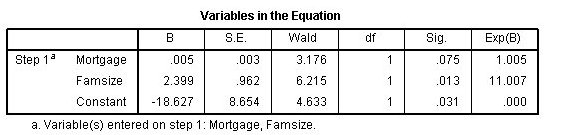
\includegraphics[scale=0.6]{images/Logistic8}\\
  \caption{Variables in the Equation}
\end{center}
\end{figure}

The \textbf{\textit{Exp(B)}} column in the table presents the extent to which raising the corresponding measure by one unit influences the odds ratio. We can interpret \textbf{\textit{Exp(B)}}) in
terms of the change in odds. If the value exceeds 1 then the odds of an outcome occurring increase; if the figure is less than 1, any increase in the predictor leads to a drop in
the odds of the outcome occurring. For example, the \textbf{\textit{Exp(B)}} value associated with
family size is 11.007. Hence when family size is raised by one unit (one person) the
odds ratio is 11 times as large and therefore householders are 11 more times likely to
belong to the take offer group.

The \textbf{\textit{B}} values are the logistic coefficients that can be used to create a predictive
equation (similar to the b values in linear regression) formula seen previously.
\begin{figure}
\begin{center}
  % Requires \usepackage{graphicx}
  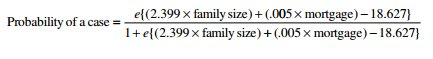
\includegraphics[scale=0.75]{images/Logistic11}\\
  \caption{Logistic Regression Equation}
\end{center}
\end{figure}

Here is an example of the use of the predictive equation for a new case. Imagine a
householder whose household size including themselves was seven and paying
a monthly mortgage of $2,500$ euros. Would they take up the offer, i.e. belong to category 1?
Substituting in we get:
\begin{figure}
\begin{center}
  % Requires \usepackage{graphicx}
  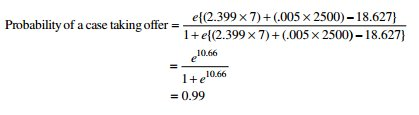
\includegraphics[scale=0.75]{images/Logistic12}\\
  \caption{Logistic Regression Equation : Example}
\end{center}
\end{figure}

Therefore, the probability that a householder with seven in the household and a mortgage of 2,500 p.m. will take up the offer is 99\%, or 99\% of such individuals will be
expected to take up the offer.
Note that, given the non-significance of the mortgage variable, you could be justified
in leaving it out of the equation. As you can imagine, multiplying a mortgage value by
B adds a negligible amount to the prediction as its B value is so small (.005).

\subsection{SPSS Outout  - Block 0: Beginning Block.}
Block 0 presents the results with only the constant included
before any coefficients (i.e. those relating to family size and mortgage) are entered into
the equation. Logistic regression compares this model with a model including all the
predictors (family size and mortgage) to determine whether the latter model is more
appropriate. The table suggests that if we knew nothing about our variables and guessed
that a person would not take the offer we would be correct 53.3\% of the time.
\begin{figure}[h!]
	\begin{center}
		% Requires \usepackage{graphicx}
		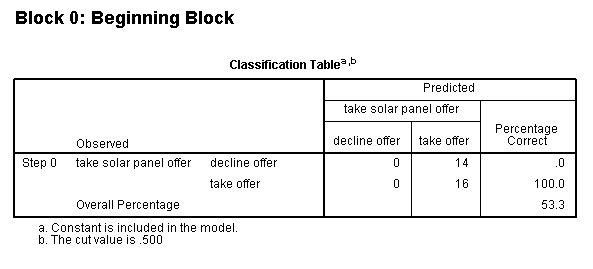
\includegraphics[scale=0.6]{images/Logistic3}\\
		\caption{Classification table}
	\end{center}
\end{figure}
The variables not in the equation table tells us whether each IV improves the model. The answer is yes for both variables, with family size slightly better than mortgage size, as both are significant and if included would add to the predictive power of the model. If they had not been significant and able to contribute to the prediction,
then termination of the analysis would obviously occur at this point

\begin{figure}
	\begin{center}
		% Requires \usepackage{graphicx}
		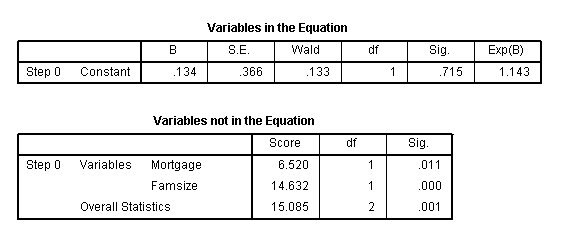
\includegraphics[scale=0.6]{images/Logistic4}\\
		\caption{Variables in / not in the equation}
	\end{center}
\end{figure}
This presents the results when the predictors �family size� and
�mortgage� are included. Later SPSS prints a classification table which shows how the
classification error rate has changed from the original 53.3%. By adding the variables
we can now predict with 90\% accuracy (see Classification Table later). The
model appears good, but we need to evaluate model fit and significance as well. SPSS will
offer you a variety of statistical tests for model fit and whether each of the independent
variables included make a significant contribution to the model.
\begin{figure}
	\begin{center}
		% Requires \usepackage{graphicx}
		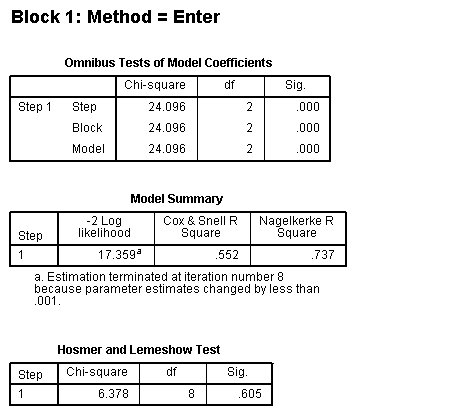
\includegraphics[scale=0.6]{images/Logistic5}\\
		\caption{Test Outcomes}
	\end{center}
\end{figure}


%The likelihood function can be thought of as a measure of how well a candidate model fits the data (although that is a very simplistic definition). The AIC criterion is based on the Likelihood function.
%The likelihood function of a fitted model is commonly re-expressed as -2LL (i.e. The log of the likelihood times minus 2).

%The difference between �2LL for the best-fitting model and �2LL for the null hypothesis model (in which all the b values are set to zero in block 0) is distributed like
%chi squared, with degrees of freedom equal to the number of predictors; this difference
%is the Model chi square that SPSS refers to. Very conveniently, the difference between �2LL values for models with successive terms added also has a chi squared distribution,
%so when we use a stepwise procedure, we can use chi-squared tests to find out if adding
%one or more extra predictors significantly improves the fit of our model.



\subsection{Logistic Regression: Decision Rule}
Our decision rule will take the following form: If the probability of the event is greater than or equal to some threshold, we shall predict that the event will take place. By default, SPSS sets this threshold to .5. While that seems reasonable, in many cases we may want to set it higher or lower than .5.
\section{SPSS Output  - Block 0: Beginning Block.}
Block 0 presents the results with only the constant included
before any coefficients (i.e. those relating to family size and mortgage) are entered into
the equation. Logistic regression compares this model with a model including all the
predictors (family size and mortgage) to determine whether the latter model is more
appropriate. The table suggests that if we knew nothing about our variables and guessed
that a person would not take the offer we would be correct 53.3\% of the time.
\begin{figure}[h!]
\begin{center}
  % Requires \usepackage{graphicx}
  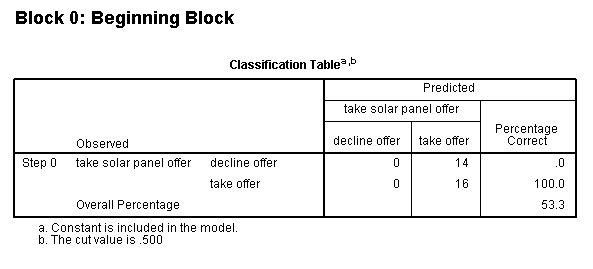
\includegraphics[scale=0.6]{images/Logistic3.jpg}\\
  \caption{Classification table}
\end{center}
\end{figure}
The variables not in the equation table tells us whether each IV improves the model. The answer is yes for both variables, with family size slightly better than mortgage size, as both are significant and if included would add to the predictive power of the model. If they had not been significant and able to contribute to the prediction,
then termination of the analysis would obviously occur at this point

\begin{figure}
\begin{center}
  % Requires \usepackage{graphicx}
  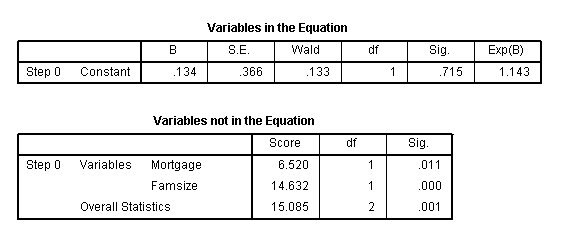
\includegraphics[scale=0.6]{images/Logistic4.jpg}\\
  \caption{Variables in / not in the equation}
\end{center}
\end{figure}
This presents the results when the predictors �family size� and
�mortgage� are included. Later SPSS prints a classification table which shows how the
classification error rate has changed from the original 53.3%. By adding the variables
we can now predict with 90\% accuracy (see Classification Table later). The
model appears good, but we need to evaluate model fit and significance as well. SPSS will
offer you a variety of statistical tests for model fit and whether each of the independent
variables included make a significant contribution to the model.
\begin{figure}
\begin{center}
  % Requires \usepackage{graphicx}
  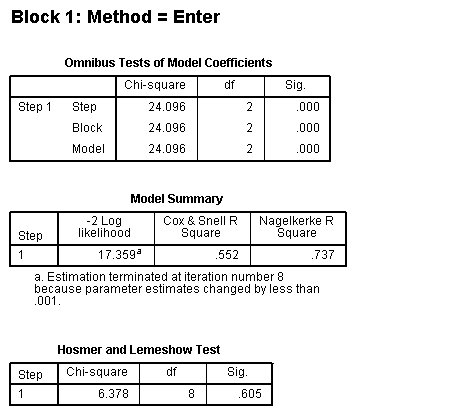
\includegraphics[scale=0.6]{images/Logistic5.jpg}\\
  \caption{Test Outcomes}
\end{center}
\end{figure}
\subsection{Omnibus Test for Model Coefficients}
The overall significance is tested using what SPSS calls the \textbf{\textit{Model Chi-square}}, which is derived from the likelihood of observing the actual data under the assumption that the model that has been fitted is accurate. There are two hypotheses to test in relation to the overall fit of the model:


 \begin{itemize}
 \item[$H_0$] The model is a good fitting model.
 \item[$H_1$] The model is not a good fitting model (i.e. the predictors have a significant effect).
 \end{itemize}
 In our case model chi square has 2 degrees of freedom, a value of 24.096 and a probability of $p < 0.000$.

Thus, the indication is that the model has a poor fit, with the model containing only the constant indicating that the predictors do have a significant effect and create essentially a different model. So we need to look closely at
the predictors and from later tables determine if one or both are significant predictors.

This table has 1 step. This is because we are entering both variables and at the same
time providing only one model to compare with the constant model. In stepwise logistic regression there are a number of steps listed in the table as each variable is added or
removed, creating different models. The step is a measure of the improvement in the
predictive power of the model since the previous step. ( I will revert to this next class).

%The likelihood function can be thought of as a measure of how well a candidate model fits the data (although that is a very simplistic definition). The AIC criterion is based on the Likelihood function.
%The likelihood function of a fitted model is commonly re-expressed as -2LL (i.e. The log of the likelihood times minus 2).

%The difference between �2LL for the best-fitting model and �2LL for the null hypothesis model (in which all the b values are set to zero in block 0) is distributed like
%chi squared, with degrees of freedom equal to the number of predictors; this difference
%is the Model chi square that SPSS refers to. Very conveniently, the difference between �2LL values for models with successive terms added also has a chi squared distribution,
%so when we use a stepwise procedure, we can use chi-squared tests to find out if adding
%one or more extra predictors significantly improves the fit of our model.


\subsection{Model Summary Table}


The likelihood function can be thought of as a measure of how well a candidate model fits the data (although that is a very simplistic definition). The AIC criterion is based on the Likelihood function.
The likelihood function of a fitted model is commonly re-expressed as -2LL (i.e. The log of the likelihood times minus 2). The �2LL value from the Model Summary table below is 17.359.

Although there is no close analogous statistic in logistic regression to
the coefficient of determination $R^2$ the Model Summary Table provides some approximations. Cox and Snell�s R-Square attempts to imitate multiple R-Square based on �likelihood�, but its maximum can be (and usually is) less than 1.0, making it difficult to interpret. Here it is indicating that 55.2\% of the variation in the DV is explained by the
logistic model. The Nagelkerke modification that does range from 0 to 1 is a more reliable
measure of the relationship. Nagelkerke�s $R^2$ will normally be higher than the Cox and Snell measure. Nagelkerke�s $R^2$ is part of SPSS output in the �Model Summary� table and is the most-reported of the R-squared estimates. In our case it is 0.737, indicating a moderately strong relationship of 73.7\% between the predictors and the prediction.
\newpage
\subsection{Hosmer and Lemeshow  Statistic}
An alternative to model chi square is the Hosmer and Lemeshow test
which divides subjects into 10 ordered groups of subjects and then compares the number
actually in the each group (observed) to the number predicted by the logistic regression
model (predicted). The 10 ordered groups are created based on their estimated probability; those with estimated probability below .1 form one group, and so on, up to those with probability .9 to 1.0.

Each of these categories is further divided into two groups based on the actual observed outcome variable (success, failure). The expected frequencies for each of the cells are obtained from the model. A probability (p) value is
computed from the chi-square distribution with 8 degrees of freedom to test the fit of the logistic model.

If the H-L goodness-of-fit test statistic is greater than .05, as we want for well-fitting models, we fail to reject the null hypothesis that there is no difference between observed and model-predicted values, implying that the model�s estimates fit the data at an acceptable level. That is, well-fitting models show non-significance on the
H-L goodness-of-fit test. This desirable outcome of non-significance indicates that the
model prediction does not significantly differ from the observed.

The H-L statistic assumes sampling adequacy, with a rule of thumb being enough cases so that 95\% of cells (typically, 10 decile groups times 2 outcome categories = 20 cells) have an expected frequency $>$ 5. Our H-L statistic has a significance of .605 which means that it is not statistically significant and therefore our model is quite a
good fit.
\begin{figure}[h!]
\begin{center}
  % Requires \usepackage{graphicx}
  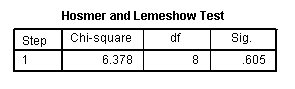
\includegraphics[scale=0.6]{images/Logistic7A}\\
  \caption{Hosmer and Lemeshow Statistic}
\end{center}
\end{figure}

\begin{figure}[h!]
\begin{center}
  % Requires \usepackage{graphicx}
  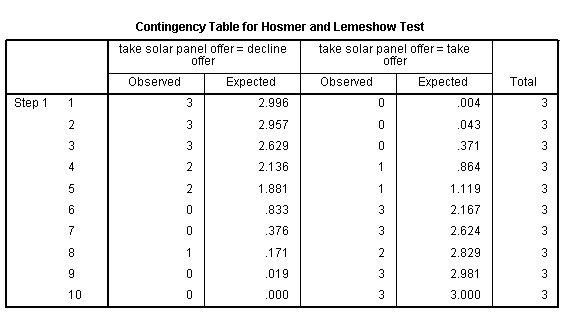
\includegraphics[scale=0.6]{images/Logistic6}\\
  \caption{Hosmer and Lemeshow Table}
\end{center}
\end{figure}
\newpage
\subsection{Classification Table}
Rather than using a goodness-of-fit statistic, we often want to look at the proportion of cases we have managed to classify correctly. For this we need to look at the classification table printed out by SPSS, which tells us how many of the cases where the observed values of the dependent variable were 1 or 0 respectively have
been correctly predicted.

In the Classification table, the columns are the two predicted values of the dependent, while the rows are the two observed (actual) values of the dependent. In a perfect model, all cases will be on the diagonal and the
overall percent correct will be 100\%. In this study, 87.5\% were correctly classified for the take offer group and 92.9\% for the decline offer group. Overall 90\% were correctly classified. This is a considerable improvement on the 53.3\% correct classification with the constant model so we know that the model with predictors is a significantly better mode.
\begin{figure}[h!]
	\begin{center}
		% Requires \usepackage{graphicx}
		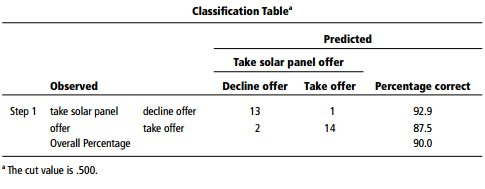
\includegraphics[scale=0.6]{images/Logistic7}\\
		\caption{Classification Table}
	\end{center}
\end{figure}
\subsection{Classification Table}
Rather than using a goodness-of-fit statistic, we often want to look at the proportion of cases we have managed to classify correctly. For this we need to look at the classification table printed out by SPSS, which tells us how many of the cases where the observed values of the dependent variable were 1 or 0 respectively have
been correctly predicted.

In the Classification table, the columns are the two predicted values of the dependent, while the rows are the two observed (actual) values of the dependent. In a perfect model, all cases will be on the diagonal and the
overall percent correct will be 100\%. In this study, 87.5\% were correctly classified for the take offer group and 92.9\% for the decline offer group. Overall 90\% were correctly classified. This is a considerable improvement on the 53.3\% correct classification with the constant model so we know that the model with predictors is a significantly better mode.
\begin{figure}[h!]
\begin{center}
  % Requires \usepackage{graphicx}
  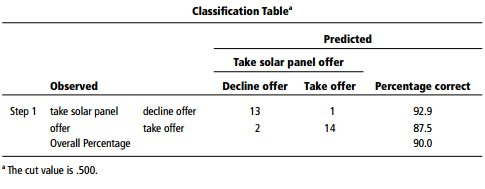
\includegraphics[scale=0.6]{images/Logistic7}\\
  \caption{Classification Table}
\end{center}
\end{figure}

\subsection{Variables in the Equation}
The Variables in the Equation table has several important elements. The Wald statistic and associated probabilities provide an index of the significance of each predictor in the equation.
The simplest way to assess Wald is to take the significance values and if less
than 0.05 reject the null hypothesis as the variable does make a significant contribution.
In this case, we note that family size contributed significantly to the prediction
(p = .013) but mortgage did not (p = .075). The researcher may well want to drop
independents from the model when their effect is not significant by the Wald statistic
(in this case mortgage).

\begin{figure}
\begin{center}
  % Requires \usepackage{graphicx}
  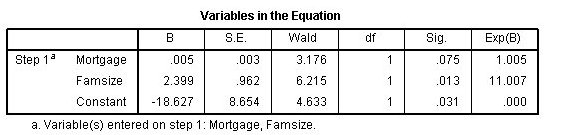
\includegraphics[scale=0.6]{images/Logistic8}\\
  \caption{Variables in the Equation}
\end{center}
\end{figure}

The \textbf{\textit{Exp(B)}} column in the table presents the extent to which raising the corresponding measure by one unit influences the odds ratio. We can interpret \textbf{\textit{Exp(B)}}) in
terms of the change in odds. If the value exceeds 1 then the odds of an outcome occurring increase; if the figure is less than 1, any increase in the predictor leads to a drop in
the odds of the outcome occurring. For example, the \textbf{\textit{Exp(B)}} value associated with
family size is 11.007. Hence when family size is raised by one unit (one person) the
odds ratio is 11 times as large and therefore householders are 11 more times likely to
belong to the take offer group.

The \textbf{\textit{B}} values are the logistic coefficients that can be used to create a predictive
equation (similar to the b values in linear regression) formula seen previously.
\begin{figure}
\begin{center}
  % Requires \usepackage{graphicx}
  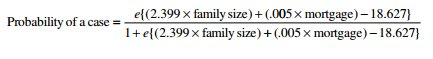
\includegraphics[scale=0.75]{images/Logistic11.jpg}\\
  \caption{images/Logistic Regression Equation}
\end{center}
\end{figure}

Here is an example of the use of the predictive equation for a new case. Imagine a
householder whose household size including themselves was seven and paying
a monthly mortgage of $2,500$ euros. Would they take up the offer, i.e. belong to category 1?
Substituting in we get:
\begin{figure}
\begin{center}
  % Requires \usepackage{graphicx}
  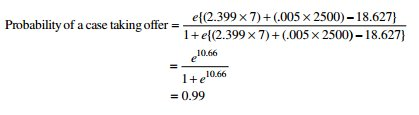
\includegraphics[scale=0.75]{images/Logistic12.jpg}\\
  \caption{images/Logistic Regression Equation : Example}
\end{center}
\end{figure}

Therefore, the probability that a householder with seven in the household and a mortgage of 2,500 p.m. will take up the offer is 99\%, or 99\% of such individuals will be
expected to take up the offer.
Note that, given the non-significance of the mortgage variable, you could be justified
in leaving it out of the equation. As you can imagine, multiplying a mortgage value by
B adds a negligible amount to the prediction as its B value is so small (.005).
\newpage

\subsection{Variables in the Equation}
The Variables in the Equation table has several important elements. The Wald statistic and associated probabilities provide an index of the significance of each predictor in the equation.
The simplest way to assess Wald is to take the significance values and if less
than 0.05 reject the null hypothesis as the variable does make a significant contribution.
In this case, we note that family size contributed significantly to the prediction
(p = .013) but mortgage did not (p = .075). The researcher may well want to drop
independents from the model when their effect is not significant by the Wald statistic
(in this case mortgage).

\begin{figure}
	\begin{center}
		% Requires \usepackage{graphicx}
		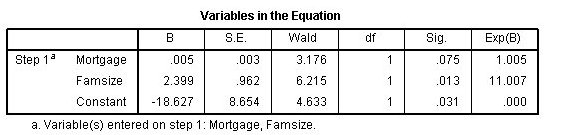
\includegraphics[scale=0.6]{images/Logistic8}\\
		\caption{Variables in the Equation}
	\end{center}
\end{figure}

The \textbf{\textit{Exp(B)}} column in the table presents the extent to which raising the corresponding measure by one unit influences the odds ratio. We can interpret \textbf{\textit{Exp(B)}}) in
terms of the change in odds. If the value exceeds 1 then the odds of an outcome occurring increase; if the figure is less than 1, any increase in the predictor leads to a drop in
the odds of the outcome occurring. For example, the \textbf{\textit{Exp(B)}} value associated with
family size is 11.007. Hence when family size is raised by one unit (one person) the
odds ratio is 11 times as large and therefore householders are 11 more times likely to
belong to the take offer group.

The \textbf{\textit{B}} values are the logistic coefficients that can be used to create a predictive
equation (similar to the b values in linear regression) formula seen previously.
\begin{figure}
	\begin{center}
		% Requires \usepackage{graphicx}
		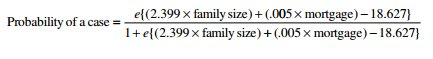
\includegraphics[scale=0.75]{images/Logistic11}\\
		\caption{Logistic Regression Equation}
	\end{center}
\end{figure}

Here is an example of the use of the predictive equation for a new case. Imagine a
householder whose household size including themselves was seven and paying
a monthly mortgage of $2,500$ euros. Would they take up the offer, i.e. belong to category 1?
Substituting in we get:
\begin{figure}
	\begin{center}
		% Requires \usepackage{graphicx}
		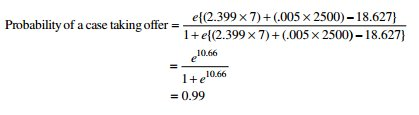
\includegraphics[scale=0.75]{images/Logistic12}\\
		\caption{Logistic Regression Equation : Example}
	\end{center}
\end{figure}

Therefore, the probability that a householder with seven in the household and a mortgage of 2,500 p.m. will take up the offer is 99\%, or 99\% of such individuals will be
expected to take up the offer.
Note that, given the non-significance of the mortgage variable, you could be justified
in leaving it out of the equation. As you can imagine, multiplying a mortgage value by
B adds a negligible amount to the prediction as its B value is so small (.005).

\end{document}

\end{document}
